\section{Vissim Network Modelling}
\label{modelling}
The Vissim network used throughout the project is derived from a network originally started COWI and later reworked by DTU Transport students.

COWI's version included O3 from Jyllingevej to the intersection with highway 3 and even further north. In addition highway 3, which runs almost parallel with O3 in this area, was included as well as the minor roads in between.
The network was setup with dynamic assignment of traffic.

\subsection{Modifications \& Additions to Existing Model}

As such the network was missing four intersections of O3 from Jyllingevej to Roskildevej. To establish this section satellite photos from Google Earth was combined with intersection layouts, kindly provided by DRD.

The signal plans and naming conventions for the existing intersections in the COWI model for O3 intersections were adopted when entering the four missing intersections into the network. As for the intersection layout, DRD provided the missing signal plans for these intersections as well.

To prevent side-effects all links not connected to O3 from Herlev Sygehus to Jylligevej were removed as well as all parking lots (DTA zones).

A number of mistakes were corrected in the definition of the intersections. This was done using layout plans for the intersections, provided by DRD. Most mistakes were related to non-existent turning-lanes (and even turning possibilities) and the placement of bus-only lanes. 

\subsection{Link Inputs}

Due to the arterial nature of the Herlev area there is a natural distinction between major and minut link inputs. The major inputs are positioned in the ends and minor inputs are placed for each minor road.

In the southgoing direction vehicles entering the arterial from highway 3 and the northern extension of O3 are represented by a single input positioned before the intersection at Herlev Sygehus and would be detected by D3.

Northgoing traffic input is defined on the link leading to the Mileparken intersection and is detected by D14. 

The relative size of the major inputs are set according to the relative directional distribution seen in Figure \ref{fig:herlev_props} ie. 45\% northgoing and 55\% southgoing. XXX Insert more specific figure XXX

As the available dataset does not include detectors on the minor sideroads - from either side of the arterial - it is difficult to assess the relative size of the inputs from them. Thus for the remaining roads adjacent to the arterial are defined minor input links of identical size with the exception of the Herlev Sygehus link, which is set to be double the size to match the observations made above.
It is arguable that much traffic enters at the Herlev Hovedgade intersection, but the detected traffic does not indicate that this is significant.

The combined traffic input is set so that in total 20\% arise from the minor roads and the remainder enters from the ends of the arterial. 

XXX Try to find something to back this up eg. from Steen Lauritzens report XXX.

\subsection{Routes}
\label{routefractions}
In the network there exist a large number of routes which road users may take. The most obvious routes go all the way through the arterial but other likely routes go from a heavy-traffic minor-road such as Herlev Hovedgade and exit at either at one of the ends of the arterial or at another heavy-traffic minor-road such as Jyllingevej.

At every intersection it is possible to follow each adjacent link (ie. turn left, right or go straight through) and thus the total number of routes from an input link to an exit link in the network is tremendous.

DRD provided traffic counts for every intersection except Ejby Torvevej (which is a blinded minor road and of little importance according to DRD) which has made it possible to model in detail the turning motions in the network.
The counting period was 7.00-9.00 in the mornings and 15.00-17.00 in the afternoons in 15-minutes intervals. The counts involved, for each approach, the turning movements of cars (including vans) and trucks. 

To apply this dataset in Vissim it is possible to use \textit{turning decisions} but the Vissim manual is clear that static routes should be used (rather than turning decisions) when modelling turning distributions. The main reason is that congestion may cause a decision to turn to be overruled whereas a vehicle on a fixed route will wait for the congestion to clear. 

The simplest approach was to introduce a routing decision for each approach, which had traffic count data, and then add routes - respecting the counting data - which represented the turning motion. Such a route is \textit{internal} as it does not necessarily lead from an input to an exit link. Consequently this approach yields a network with the possibility of endless circulation, however since we only regard an arterial in this project - and the fact that there are no U-turns in the network - no vehicles will be able to circulate and will always find an exit link.

The routing decision must be placed at a \textit{decision point}, however this does not exist in Vissim. Rather the decision point is scattered over 2 or more connectors attached to each link facing an intersection. In order to overcome this these connectors were grouped by a naming convention which identifies which decision point they belong to and which turning motion they will cause a vehicle to take. 
The names are the concatenation of the direction from which traffic arrives (ie. north, south, east or west), the number of the intersection the decision belongs to (intersections are numbered increasingly from north to south) and finally the turning motion (ie. left, through or right), whichever is applicable. 

As an example the decision point at Herlev Sygehus (intersection 1), which faces traffic from north consist of three connectors, are called \verb|N1L|, \verb|N1T| and \verb|N1R|.

To find the insertion point for the routing a backtracking search is made from each turning motion until a common link is found. This link is thus the decision point and we can automatically generate our internal routes by using the discovery routine of section \ref{routingdecisions} to find a valid route.

In Figure \ref{fig:flow_dist_principle} is an example of decision points (y) and the proportions of traffic for each turning motion.
\begin{figure}[!ht]
\begin{center}
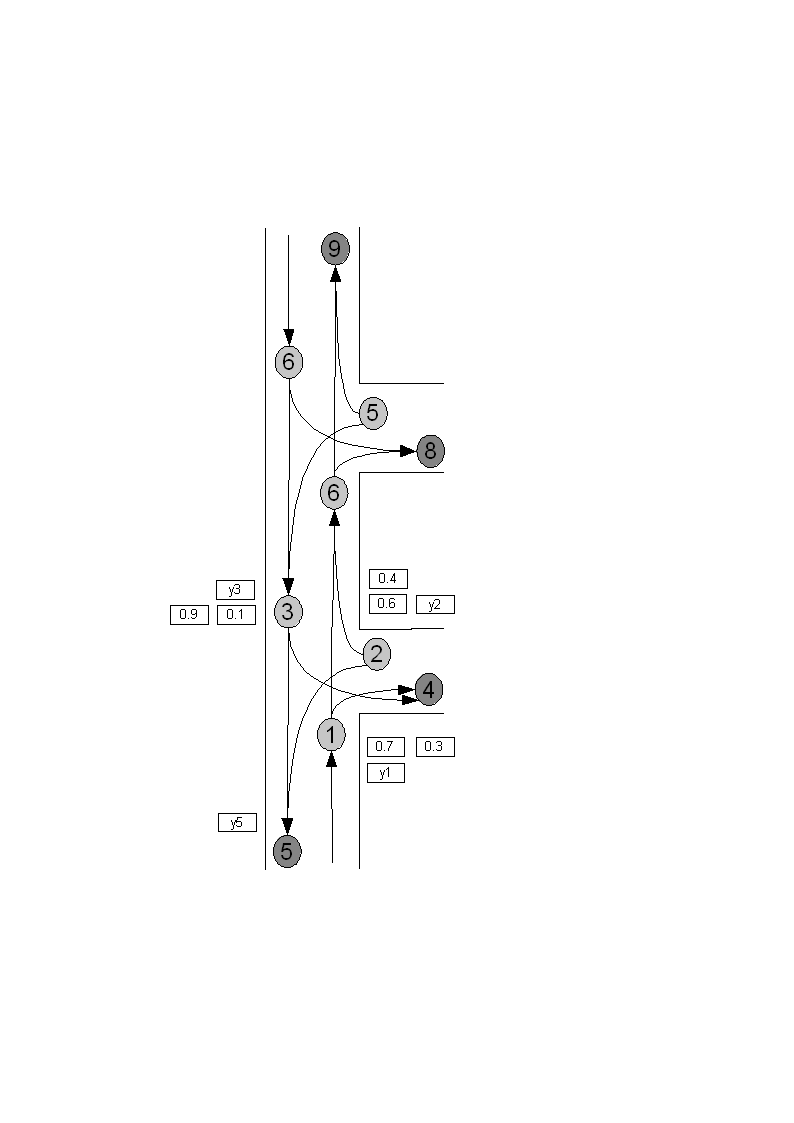
\includegraphics[scale=0.6]{trafficcount_to_routes_sketch.png} 
\end{center}
\caption{Flow distribution principle}
\label{fig:flow_dist_principle}
\end{figure}

\subsection{Signal Plans}
Signal plans define the stage sequence, green duration and how changes between adjacent stages should happen with respect to colors in the from and to stages. For cycle-based signal plans the cycle time must be equal to the sum of green and interstage time from the beginning of the first stage until it begins again.

A single stage defines the signal head colors of one or more signal group, which, in turn, is a group of signal heads operating synchronously.

The simplest signal controller consist of two stages. In  Figure \ref{fig:simple_intersection} the arrows indicate the directions being served green.

\begin{figure}[!ht]
\begin{center}
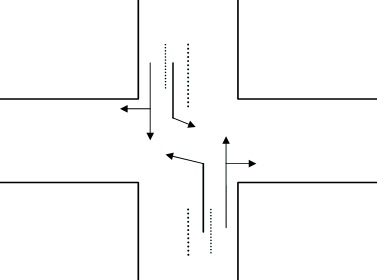
\includegraphics[scale=0.5]{simple_intersection.png} 
\end{center}
\caption{A simple intersection}
\label{fig:simple_intersection}
\end{figure}

DOGS rely on existing signal and modify the duration of the stage or stages, which serve green in the direction of the arterial. Thus DOGS assume that the stage sequence and interstages are \textit{optimized} so that the time lost in stage changes is minimized and \textit{safe} so that vehicles in eg. left-turning movements have time to leave the intersection before the conflicting direction receives green.

For this project DRD has supplied a number of signal plans for each intersection, developed by TTS. Throughout the plans signal groups in one direction (usually the major one) are named A and B in the perpendicular direction. Names such as At, Av, AtV indicates signal group for the throughgoing, leftgoing (V = venstre (danish) = left) and a combination for the final name variant. Lower case a's and b's indicate a signal group for pedestrians in the major and minor direction resp. Lower case v's mean that for the controller(s) in this plan a left-turning light is attached to an ordinary red-yellow-green light in order to make it clear that left-turners now have the lane to themselves. If the V is in upper case the light is exclusively for left-turning traffic.

For some intersections a number of alternative plans were supplied. Considering the scope of this project only a single plan was chosen for each intersection and time of day. Generally plans involving pedestrian or bicyclist actuated stages were avoided so as to maximize the potential for traffic signal optimization. It was confirmed by TTS that these types of stages, which are taken in a stochastic manner ie. when a button is pressed, can be devastating to the coordination of traffic signals.

As a final simplifying step it was chosen not to provide signal heads for pedestrians and bicyclists as these types of road users are not being simulated. Pedestrian stages will mostly follow the parallel stages anyway and if this is not the case the stage, which is being denied in favor of the pedestrian stage, will simply receive red for the duration.

The final plans, which are used in the simulation, can be seen in appendix \ref{app:signalplans}.

The actual implementation was done in VAP by running the interstages at the cycle second according to the signal plan, for more details refer to section \ref{vap}.

\subsection{Signal Controller Details}
\label{signal_details}
The optimization system (see Section \ref{eval_coord}) needs some additional information on the signal controllers, the distances between intersections and which stages are arterial. This is not immediately available in the Vissim network file but can be deduced.

Since Vissim does not offer the concept of an intersection - and this is needed to place intersections relative to each other for signal coordination - this information was extracted as follows.

Arterials have the property that they have two major traffic streams, which traverse the arterial from end to end. These streams can be called \textit{up and down} or \textit{left and right} or even \textit{clockwise and counterclockwise}. The point is that there are always two. In this project the streams were called North and South indicating the direction from which they come. We can now find these streams by finding the routes that traverse all decisions (see Section \ref{routefractions}), which are through-going and in one of the arterial directions.

For the arterial route from north, we look for a route which reaches the Herlev Sygehus intersection from north and takes the throughgoing turning option \verb|N1T|, the route must then pass through Hjortespringvej \verb|N2T| and so forth until it takes the final decision at Roskildevej \verb|N12T| and exit the network.

\subsubsection*{Distances between intersections}
One of the things we really need to assess the quality of coordinations is the distances between the signal heads (stop-line) for adjacent intersections. The Vissim network file contains information on which link or connector (abbr. road segement) each head is placed. By marking all road segments, which are part of the arterial routes, we can deduce which signal heads give green light vehicles travelling in the arterial direction.

The distance from signal controller 1 to 2 is then calculated by summing the lengths of road segments from the arterial signal heads at controller 1 to the arterial heads at controller 2.

\subsubsection*{Arterial stages}
This is also a good time to mention the notion of arterial stages. In optimization of coordinations we need to know if a stage is meant for the arterial or for a minor road. And if it is for the arterial, from which direction?

When we calculated distances between intersections on the arterial we learned which signal heads provided for the artery. Since each head is a part of a signal group and a stage is a selection of groups, which are run simultaneously, we can deduce the arterial stages using these rules:

\begin{enumerate}
\item A stage is arterial ie. gives green light to the artery, if it contains an \textit{arterial group}
\item A group is arterial if it contains an arterial signal head
\item And finally, as outlined previously, a signal head is arterial if is placed as on a link, which is marked as arterial
\end{enumerate}

The reason I only require stages and groups to \textit{contain} an arterial group and head resp. is that a stage could contain purely arterial groups and then, maybe, a group for left-turners but the stage is still arterial.

During group naming, when intersections are built, the designers usually prefix the name of the main direction \verb|A| and the side roads \verb|B|. By extracting the definitions of arterial groups as explained above we can see that not all road engineers had the same opinion:

\begin{table}[!ht]
\begin{center}
\begin{tabular}{l|l|l}
 & \textbf{Intersection} & \textbf{Arterial Groups}\\ \hline
1 & Herlev Sygehus & A1, A2\\
2 & Hjortespringvej & A, At\\
3 & Herlev Bygade & A, At\\
4 & Herlev Hovedgade & B, Bt\\
5 & Mileparken & A, At\\
9 & Fabriksparken & A1, A2\\
10 & Gammel Landevej & A1, A2\\
11 & Kindebjergvej & A1, A2\\
12 & Roskildevej & B, Bt\\
\end{tabular}
\end{center}
\caption{Groups for main traffic direction as perceived by traffic signal designer}
\label{tab:arterial_groups}
\end{table}

As can be seen in Table \ref{tab:arterial_groups} the perceived main directions for Herlev Hovedgade and Roskildevej is to-and-fro the city of Copenhagen and western Sealand.
